\label{app.01}
%\appendix
\chapter*{Prílohy}
\markboth{Prílohy}{}
\addcontentsline{toc}{chapter}{Prílohy}
\renewcommand{\thesection}{\Alph{section}}

% ======== DOKUMENTACIA ======= %
\section{Technická dokumentácia}\label{tech-doku}
\textit{Obsah elektronického média}
\begin{itemize}
	\item \textit{Thesis.pdf} obsahuje elektronickú verziu tejto práce.
	\item Adresár \textit{moa-hfdt-extension} obsahuje rozšírenie nástroja MOA a experimenty, ktoré boli doteraz vykonané.
	\item Adresár \textit{vis} obsahuje prototyp vizualizácie so vzorovými súbormi.
	\item Adresár \textit{prototype} obsahuje prototyp webového rozhrania pre vizualizáciu.
\end{itemize}

\textit{Návod na inštaláciu}
\begin{itemize}
	\item Pre spustenie vizualizácie je potrebné povoliť v prehliadači cross-origin zdroje. Následné stačí dvojklikom spustiť súbor \textit{tree.html}.
	\item Pre spustenie experimentov je potrebné nainštalovať IDE Intellij\footnote{https://jetbrains.com/} a importovať adresár \textit{moa-hfdt-extension} ako nový projekt. Importovaný projekt bude obsahovať všetky potrebné nastvenia pre spustenie.
\end{itemize}



\newpage
\section{Plán zimného semestra 2016/2017}\label{plan-zima}
\begin{itemize}
	\item Rozšírenie analýzy o ďalšie metódy a celkovo zpresnenie, zprehľadnenie a orezanie analýzy.
	\item Dokončenie návhu vlastnej metódy.
	\item Implementácia metódy.
	\item Evaluácia metódy - toto je priamo súčasťou navrhovanej metódy.
	\item Príprava článku na nejakú konferenciu, napr. IIT.SRC.
	\item Prvý experiment s použitím Eye Tracker-a na evaluáciu vizualizácie výsledkov.
\end{itemize}

\paragraph{Vyjadrenie k plneniu plánu zimného semestra} Jedným z cieľov zimného semestra bolo rozšírenie analýzy. Môžme objektívne tvrdiť, že sa nám úspešne podarilo splniť tento cieľ. Časť analýzy projektu bola značne prehĺbená a rozšírená.
\par
Ďalším cieľom bolo dokončenie návrhu vlastnej metódy. Postupne a iteratívne sme celý semester pracovali na splnení tohto cieľa. Dnes, na konci zimného semestra máme presnú predstavu o tom ako má nami navrhovaná metóda vyzerať. Toto tvrdenie podporuje aj stav kapitoly \ref{Klasifikácia rozhodovacími stromami}.
\par
Navrhovaná metóda bola implementovaná ako prvý prototyp. Tento prototyp ešte z ďaleka nepredstavuje finálnu verziu implementácie. Avšak, pomohol nám realizovať prvé jednoduché experimenty a teda aj výsledky, ktoré sú opäť prezentované v práci. Podarilo sa nám tiež implementovať prototyp, ktorý má jednoducho interpretovať a vizualizovať výsledky metódy požívateľovi.
\par
Síce sme implementovali prvé prototypy, evaluácia metódy bola len veľmi jednoduchá a základná. Napríklad nepodarilo sa nám splniť jeden zo stanovených cieľov - prvý experiment s použitím EyeTracker-a alebo používateľská štúdia.

\newpage

\section{Plán letného semestra 2016/2017}\label{plan-leto}
Tento plán popisuje náš plán ďalšieho vývoja diplomovej práce v nasledujúcom letnom semestri na týždennej granularite. Pričom predpokladáme, že semester má 12 týždňov.
\begin{itemize}
	\item \textit{1-2 týžden}: Príprava článku na študentskú vedeckú konferenciu IIT.SRC. V prvých dvoch týždňoch semestra sa chceme sústrediť na dokončenie vyhodnotenie experimentov. Tieto výsledky chceme prezentovať na IIT.SRC, preto bude tomuto potrebné venovať viac času.
	\item \textit{3 týždeň}: Vyhodnotenie prezentovaných výsledkov na IIT.SRC, určenie ďalšieho smeru a priestoru na zlepšenie aktuálneho stavu implementovanej metódy.
	\item \textit{4. týždeň}: Implementácia návrhov na zlepšenie metódy pre klasifikáciu a ich vyhodnotenie.
	\item \textit{5. týždeň}: Implementácia návrhov na zlepšenie metódy pre vizualizáciu a ich vyhodnotenie. 
	\item \textit{6. týždeň}: Vyhodnotenie kvality a výkonnosti implementovanej metódy - kvantitatívne vyhodnotenie stanovených metrík kvality.
	\item \textit{7. týždeň}: Návrh ďalších experimentov vo forme používateľskej a expertnej štúdie v použiteľnosti navrhovanej metódy.
	\item \textit{8. týždeň}: Používateľská štúdia a spísanie výsledkov kvantitatívných metrík kvality metódy z 5-6. týždňa.
	\item \textit{9. týždeň}: Vyhodnotenie používateľskej štúdie.
	\item \textit{10. týždeň}: Analýza priestoru na zlepšenie navrhovanej a implementovanej metódy podľa výsledkov používateľskej štúdie.
	\item \textit{11. týždeň}: Spísanie výsledkov používateľskej štúdie a finalizácia diplomovej práce, príprava na odovzdanie.
	\item \textit{12. týždeň}: Odovzdanie diplomovej práce.
\end{itemize}

\paragraph{Vyjadrenie k plneniu plánu letného semestra} V tomto semestri sme mali stanovené dva hlavné ciele: publikovanie článku na študentskej vedeckej konferencii IIT.SRC 2017 a kvalitatívne vyhodnotenie vizualizácie. 
\par
V prvých dvoxh týždňoch sme využili na dokončenie článku na konferenciu IIT.SRC. Náš článok bol prijatý a úspešne prezentovaný na tejto študentskej vedeckej konferencii. Počas týchto prvých dvoch týždňov sme sa chceli venovať najmä na vyhodnoteniu experimentov. Prvé experimenty sa nám podarilo spraviť a vyhodnotiť, ale nebolo to v takom rozsahu aký sme pôvodne plánovali.
\par
V štvrtom a piatom týždni sme sa sústredili na implementáciu návrhov na zlepšenie metódy vizualizácie. V tomto čase sme sa venovali hlavne zbierani návrhov a zlepšení vizualizácie. Vylepšenia boli implementované len čiastočne.
\par
V šiestom týždni sme podľa plánu vykonali kvalitatívne experimenty s cieľom overenia výkonnosti nami aplikovanej metódy rozhodovacích stromov.
\par
Ďalšia implementácia vylepšení vizualizácie a návrh používateľskej štúdie prebiehal v siedmom až ôsmo týždni, čo je posunutie o dva týždne oproti pôvodnému plánu. Používateľskú štúdiu sme vykonali až v desiatom týždni semestra, čo je rovnako dvojtýždňový posun oproti plánu.
\par
Napriek dvojtýždňovému posunu implmentácie vylepšení vizualizácie a experimentu používateľskou štúdiou sme v posledných dvoch týždňoch úspešne vyhodnotili výsledky experimentov. Prácu odovzdávame v 13. týždni namiesto plánovanému 12. týždňu.
\par
Celkovo hodnotíme plnenie plánu ako dostatočné. Napriek oneskoreniu pri plnení niektorých bodov plánu sa nám úspešene podarilo splniť všetky cieľe stanovené pre tento semester.

\newpage

\section{Článok prezentovaný na konferencii IIT.SRC 2017}
Článok, ktorý vznikol z tejto diplomovej práce bol prijatý na študentskú vedeckú konferenciu IIT.SRC 2017. Na tejto konferencii sme článok prezentovali s posterom v bloku Intelligent Information Processing. Pôvodné úplné znenie článku je zobrazené od nasledujúcej strany.
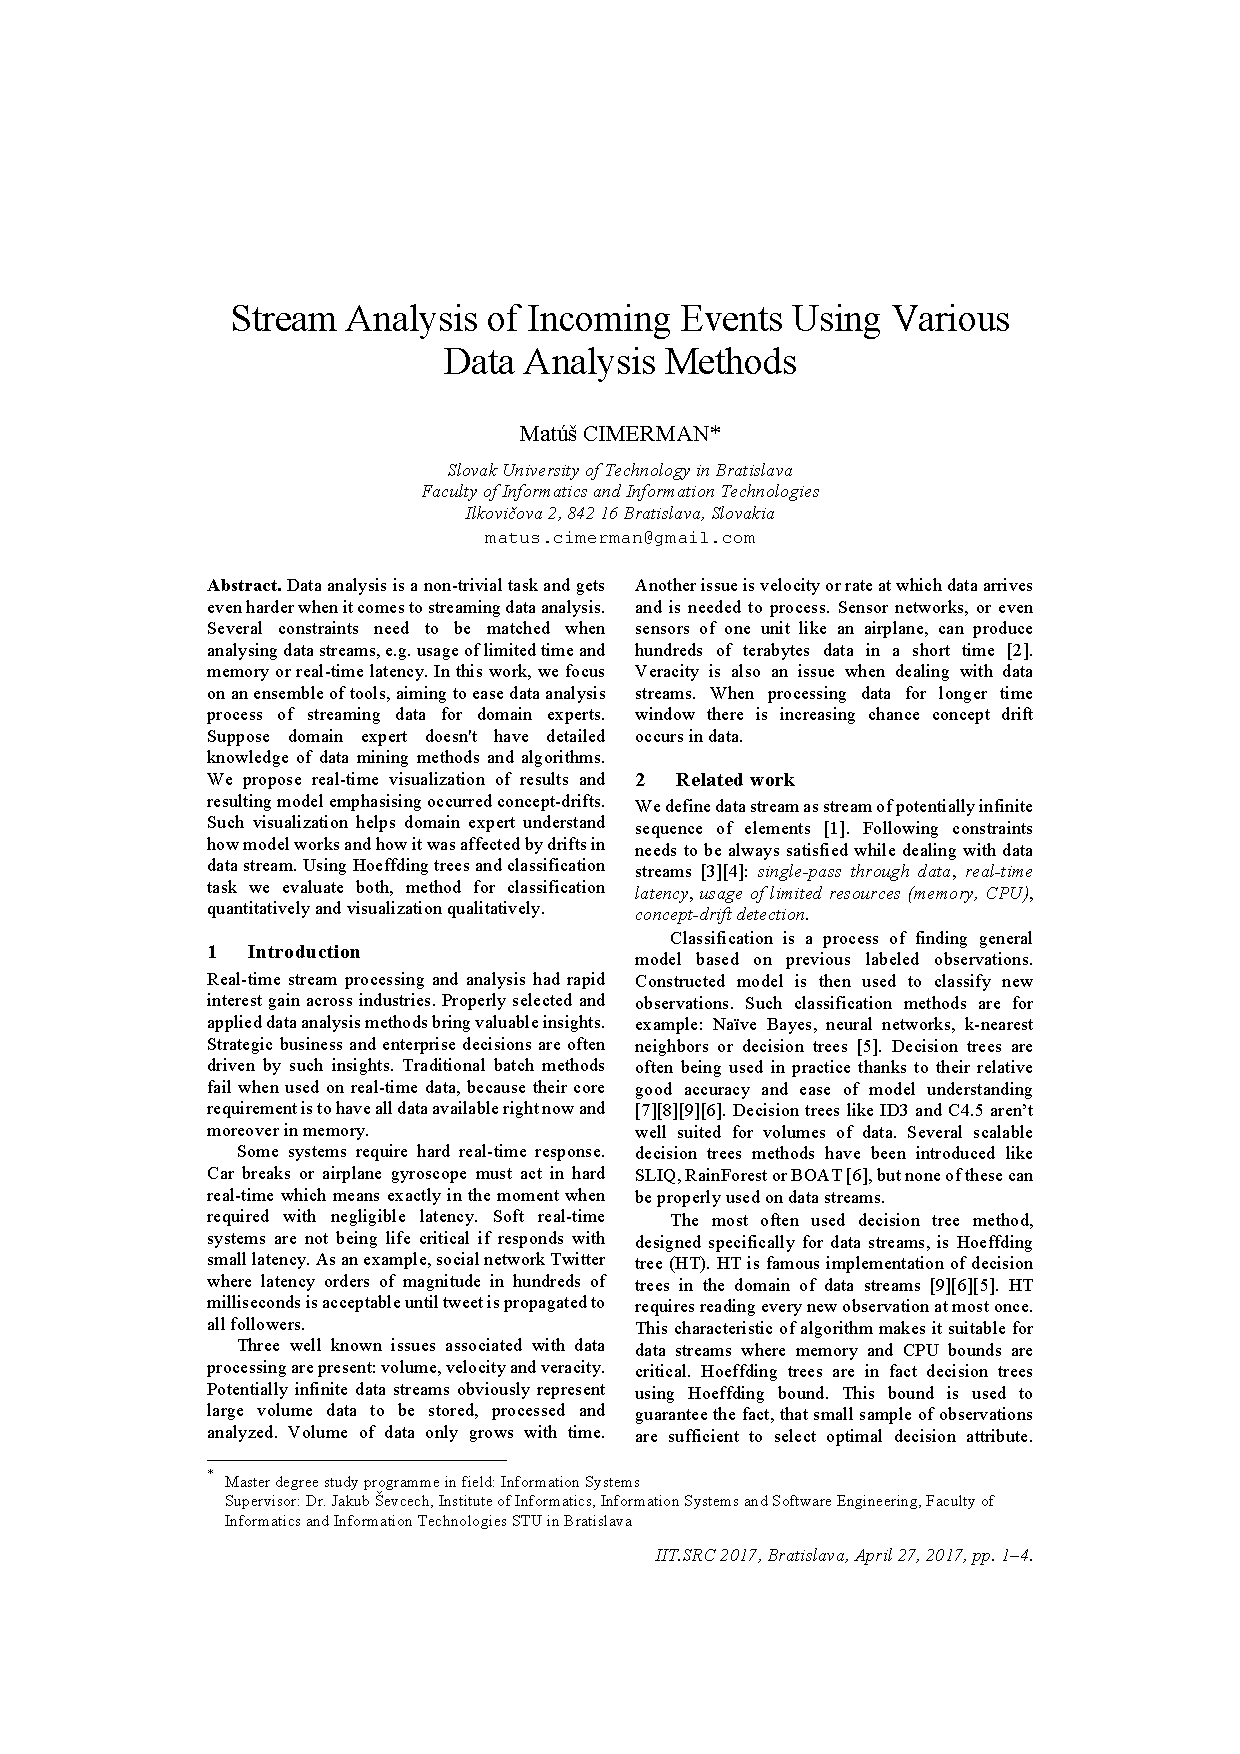
\includepdf[pages={1,2,3,4}]{IITSRC2017_paper_17.pdf}










